\documentclass[tikz,fontsize=8pt]{standalone}
\usepackage{fourier}
\usetikzlibrary{arrows.meta}
\usetikzlibrary{calc}
\tikzset{>=latex}
\definecolor{bookblue}{RGB}{0,173,239}
\definecolor{bookpink}{RGB}{236,0,140}
\definecolor{bookgreen}{RGB}{50,200,0}
\definecolor{bookbluearea}{RGB}{204,239,252}
\tikzstyle{blueline}=[draw=bookblue,line width=0.2mm]
\tikzstyle{pinkline}=[draw=bookpink,line width=0.2mm]
\tikzstyle{greenline}=[draw=bookgreen,line width=0.2mm]
\tikzstyle{blackline}=[draw=black,line width=0.2mm]
\tikzstyle{bluearea}=[fill=bookbluearea]

\usepackage{scrextend}
\changefontsizes[8pt]{8pt}
\usetikzlibrary{decorations.pathreplacing, calc}
\begin{document}
  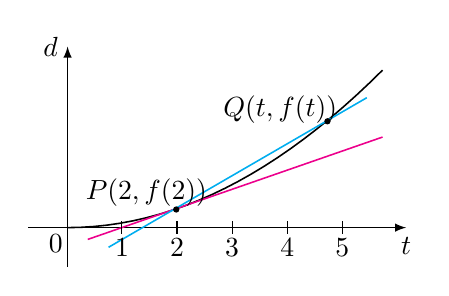
\begin{tikzpicture}
    \node at (-0.15,-0.2) {0};
    \draw[->] (-0.5,0) -- (4.3,0) node[below] {$t$};
    \draw[->] (0,-0.5) -- (0,2.3) node[left] {$d$};
    
    \draw[blackline,domain=0:2] plot (\x*2,{.5*(\x)^2});
    \draw[pinkline] (0.256,-0.15) -- (4,1.15);
    \draw[blueline] (0.52,-0.25) -- (3.8,1.65);
    \fill (1.38,0.23) circle (0.4mm);
    \fill (3.3,1.35) circle (0.4mm);
    \node at (1,0.45) {$P(2,f(2))$};
    \node at (2.7,1.5) {$Q(t,f(t))$};
    \foreach \x in {0,...,4}{
    	\pgfmathparse{int(\x+1)}\xdef\mya{\pgfmathresult}
    	\draw (.7*\x+.69,-.08) -- (.7*\x+.69,.08);
    	\node at (.7*\x+.69,-0.25) {\mya};
    }
  \end{tikzpicture}
\end{document}